\documentclass[10pt,a4paper]{article}
\usepackage[margin=0.75in]{geometry}
\usepackage[T1]{fontenc}
\usepackage[utf8]{inputenc}
\usepackage{lmodern,microtype,graphicx,booktabs,amsmath,xcolor}
\usepackage[hidelinks]{hyperref}
\usepackage{xurl}
\setlength{\parindent}{0pt}
\setlength{\parskip}{4pt}
\setlength{\emergencystretch}{3em}
\newcommand{\us}{$\mu$s}
\begin{document}
\begin{center}
{\LARGE\bfseries Distributed Tidehunter}\\[3pt]
{\large Final Google Cloud campaign: architecture and measurements}\\[2pt]
6 November 2026
\end{center}

\section{Scope and findings}
This is a synthetic key--value benchmark, not Sui checkpoint replay. The final campaign completed 411 API cases and four native Valkey controls. It followed seven campaign attempts; only the admitted final archive supplies the final measurements. The final fleet was \texttt{bench-ce0007878bef48e8}. Each case has one independent repetition. Results describe these cases, not a general ranking or a production capacity guarantee.

\textbf{Executive findings.} The final 411 API cases and four native Valkey controls completed; the audited API populations are numerically coherent. Several orderings are suspicious and unexplained: TH verbs has a higher p50 than TH TCP in 19 of 92 matched success populations. The strongest evidence for cache-bypassed remote-storage paths is the 64 KiB cold-OS cohort and the sealed SPDK direct-I/O path. The former requests a cache drop, while the latter bypasses the target OS page cache. Neither proves every call reaches media; the per-call media-hit fraction is unmeasured.

In the 1 KiB concurrent scalar-read cases, successful API medians were 1.480 \us\ for native Tidehunter, 63.575 \us\ for Tidehunter TCP, 35.752 \us\ for verbs, 46.003 \us\ for live kernel NVMe-oF and 124.412 \us\ for live SPDK NVMe-oF. These are distinct paths and populations. A native in-process lookup, a remote owner request and a remote NVMe read do not perform the same work. Valkey GET reads RAM, not the Value WAL.

\section{Architecture and read paths}
\begin{center}
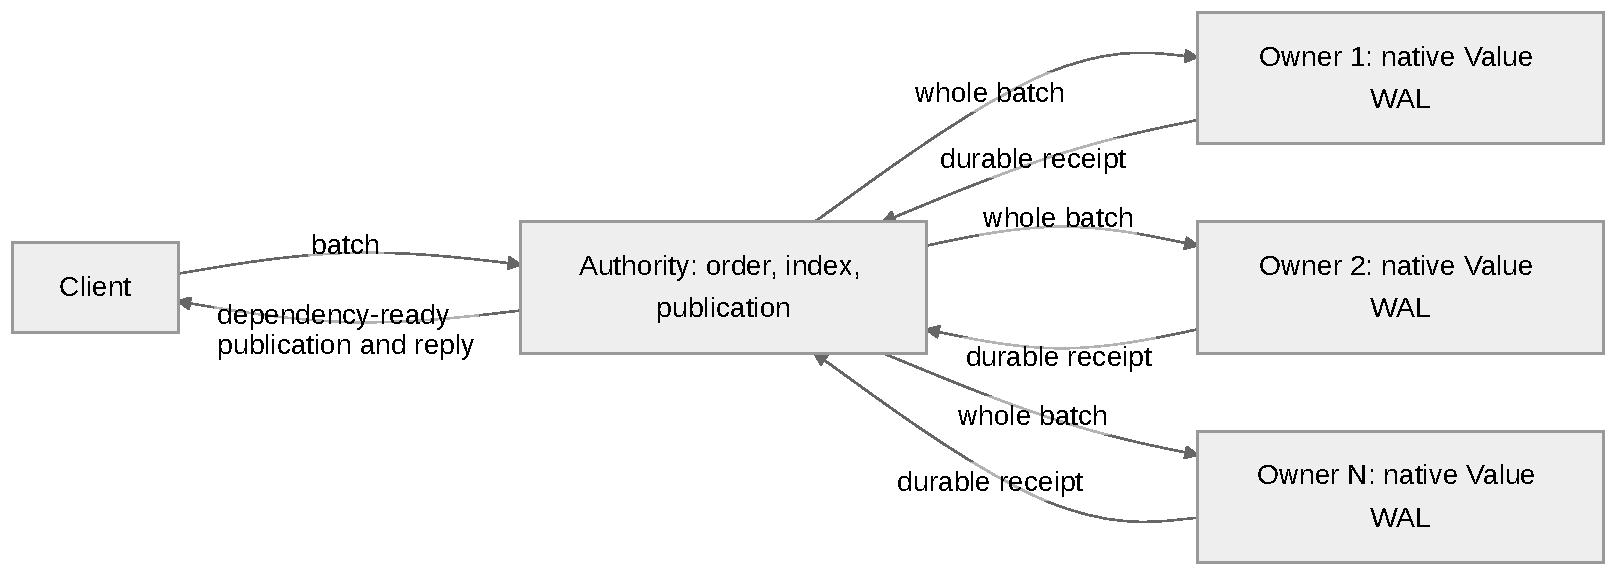
\includegraphics[width=.90\linewidth,height=1.75in,keepaspectratio]{figures/topology.pdf}\\[-2pt]
\small A whole batch goes to one owner and receives one durable receipt. Each owner has its own Value WAL; arrows do not represent replication.
\end{center}
The coordinator selects an owner, which appends and persists a batch. The coordinator publishes index entries after relevant predecessor dependencies resolve. A logical version is not a global physical WAL offset. Independent batches can overlap, and a stable checkpoint frontier advances through a contiguous resolved prefix. RF1 means one durable owner, not consensus-backed failover; permanent loss of that copy is not tolerated. General serializable transactions across independent batches are not claimed.

A coordinator-cache hit can avoid remote data traffic. On a miss, TCP and verbs request the value from the owner process, which reads its local WAL; that read can hit the owner's page cache. Registered-RAM RDMA/RMA is a different possible tier, not a direct SSD read or a measured active owner-value grant path here. NVMe-oF paths instead let the coordinator read a remote WAL over RDMA: the kernel target uses buffered file backing and the SPDK target uses direct file AIO. The sealed route reads immutable WAL; the live route addresses active WAL. Neither an RDMA label nor a cache-drop operation proves physical SSD access. The SPDK path can still encounter device caches.

\section{Method and interpretation}
Six \texttt{z4m-highmem-16} VMs in \texttt{us-central1-a} used Falcon/IRDMA, one coordinator and five storage hosts with Local SSD. The live NVMe-oF initiator explicitly requests one I/O queue at depth 32 per controller, with effective queue count 2 and \texttt{sqsize=31}. The sealed initiator uses \texttt{nvme connect} without explicit queue flags; this live policy is not established for sealed connections. Earlier host defaults were 16 by 128. RF1 aligns replica count, not semantics, cache placement, persistence or security. Valkey writes use AOF \texttt{appendfsync=always}; Tidehunter uses a different Value-WAL barrier and publication contract. Native has no network hop.

API time is completion minus dispatch; scheduling time is dispatch minus scheduled arrival; response time is completion minus scheduled arrival. Quantiles use exact nearest rank within a single operation/outcome population. A 32-value call is measured as one complete call. Rates divide successful calls by the observed case exposure, not by a steady-state interval. Rejected arrivals have no dispatched API latency and are counted separately. Percentiles are descriptive, without pooling, outlier removal, confidence intervals or run-to-run variability estimates. The benchmark reports no all-phase errors or wrong values and no timeouts or unknown mutations; this does not prove linearizability.

\section{Matched 1 KiB primary results}
Tables 1 and 2 show successful calls at concurrency 16. The first number is API p50, the second API p99 in \us, and the third is successful calls/s. Populations are 8,192 scalar reads, 4,096 scalar writes, and 2,048 calls for each batch case. Valkey write-batch32 cases were not present; a dash is not zero. See \path{evidence.json} for case IDs and exact values.
\begin{center}\small
\begin{tabular}{lrrr|rrr}\toprule
& \multicolumn{3}{c|}{Scalar read} & \multicolumn{3}{c}{Scalar write}\\
Backend & p50 & p99 & calls/s & p50 & p99 & calls/s\\\midrule
Native & 1.48 & 2.64 & 270631 & 68.73 & 169.57 & 157365\\
TH TCP & 63.58 & 283.45 & 160111 & 373.19 & 906.28 & 38490\\
TH verbs & 35.75 & 191.15 & 239334 & 361.92 & 833.53 & 39462\\
NVMe kernel live & 46.00 & 373.26 & 111589 & 1477.35 & 4323.21 & 9198\\
NVMe SPDK live & 124.41 & 380.73 & 97561 & 1525.90 & 4132.61 & 8959\\
Valkey TCP & 49.48 & 94.92 & 200965 & 177.17 & 437.99 & 78150\\
Valkey RDMA & 41.22 & 92.54 & 150160 & 172.92 & 439.61 & 80146\\\bottomrule
\end{tabular}\\[2pt] Table 1. 1 KiB scalar calls, one repetition; success-only API latency.
\end{center}
\begin{center}\small
\begin{tabular}{lrrr|rrr}\toprule
& \multicolumn{3}{c|}{Read-many32} & \multicolumn{3}{c}{Write-batch32}\\
Backend & p50 & p99 & calls/s & p50 & p99 & calls/s\\\midrule
Native & 64.49 & 103.79 & 98852 & 1148.46 & 1424.96 & 12605\\
TH TCP & 1252.11 & 3781.45 & 10868 & 2522.91 & 3561.79 & 6495\\
TH verbs & 1125.95 & 3707.76 & 11563 & 2573.46 & 3474.17 & 6426\\
NVMe kernel live & 1187.82 & 4570.25 & 10566 & 2226.34 & 3777.19 & 6636\\
NVMe SPDK live & 1332.31 & 6356.66 & 8975 & 2364.47 & 4339.40 & 6248\\
Valkey TCP & 372.69 & 797.08 & 31498 & -- & -- & --\\
Valkey RDMA & 320.67 & 788.16 & 35821 & -- & -- & --\\\bottomrule
\end{tabular}\\[2pt] Table 2. 1 KiB 32-value calls; success-only API latency, one repetition.
\end{center}

\section{Primary workload curves}
\begin{center}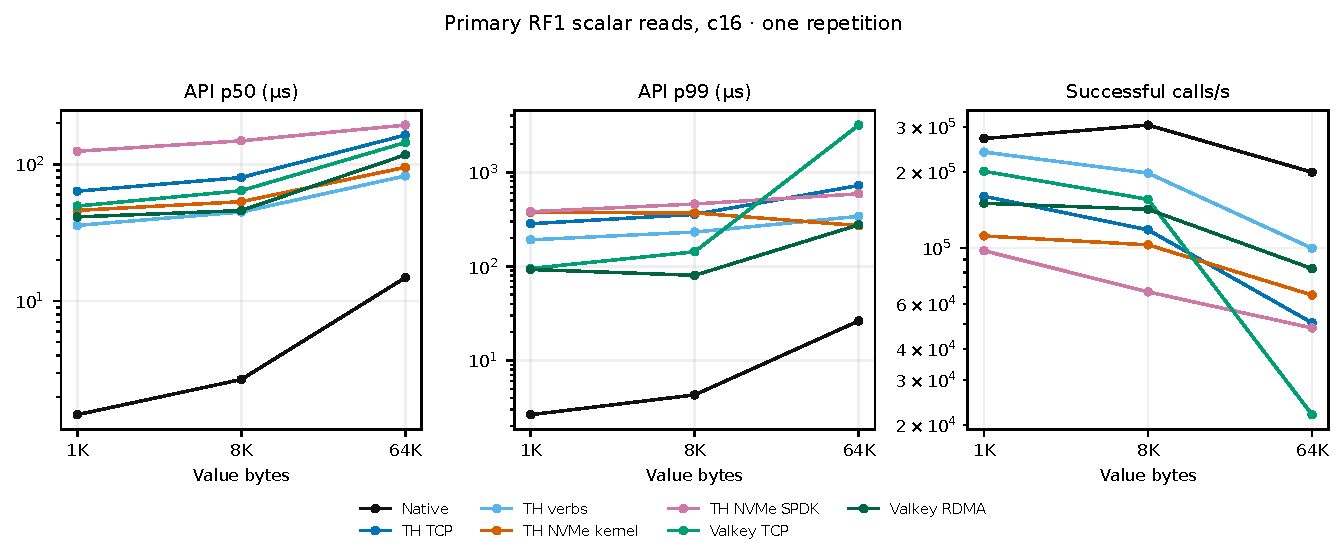
\includegraphics[width=.98\linewidth]{figures/read.pdf}\\
\small Figure 1. Primary RF1 scalar reads, c16, 8,192 successful calls per case. API p50/p99 and whole-case successful calls/s; one repetition. Coordinator cache is disabled for Tidehunter; owner and kernel-target page cache may serve reads. Valkey GET reads RAM.
\end{center}
\begin{center}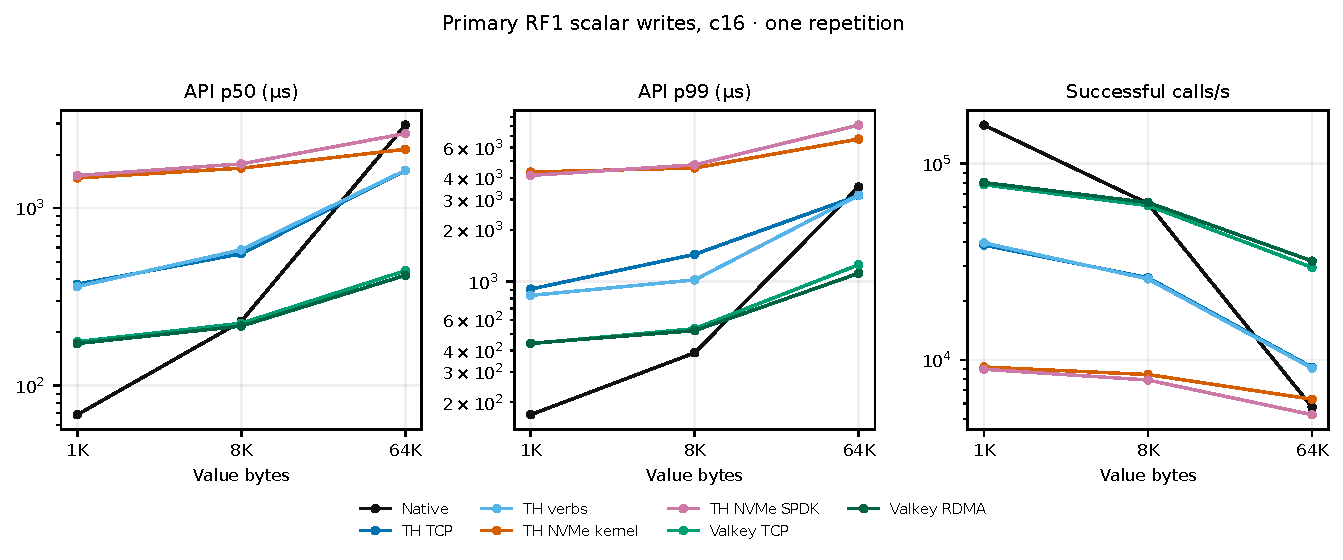
\includegraphics[width=.98\linewidth]{figures/write.pdf}\\
\small Figure 2. Primary RF1 scalar writes, c16, 4,096 successful calls per case. API p50/p99 and successful calls/s; one repetition. Tidehunter WAL barrier and Valkey AOF-always acknowledgements are different durability contracts.
\end{center}
\begin{center}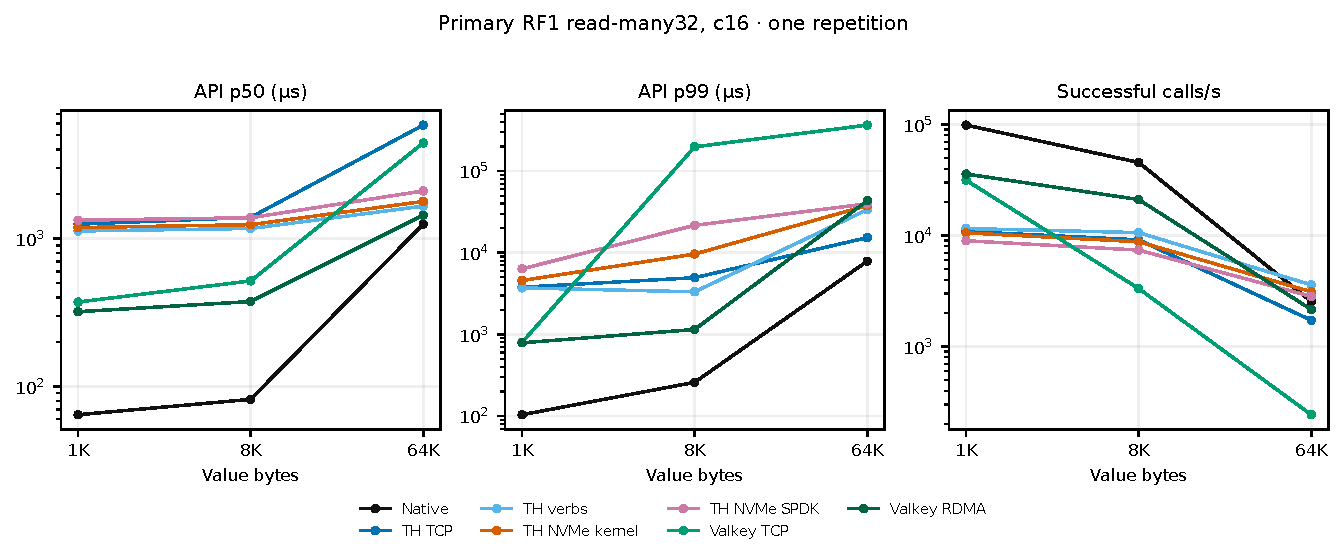
\includegraphics[width=.98\linewidth]{figures/read32.pdf}\\
\small Figure 3. Primary RF1 read-many32, c16, 2,048 successful calls per case. API p50/p99 and successful calls/s; one repetition. A call covers 32 values. Coordinator cache disabled; page cache and Valkey RAM remain relevant.
\end{center}
\begin{center}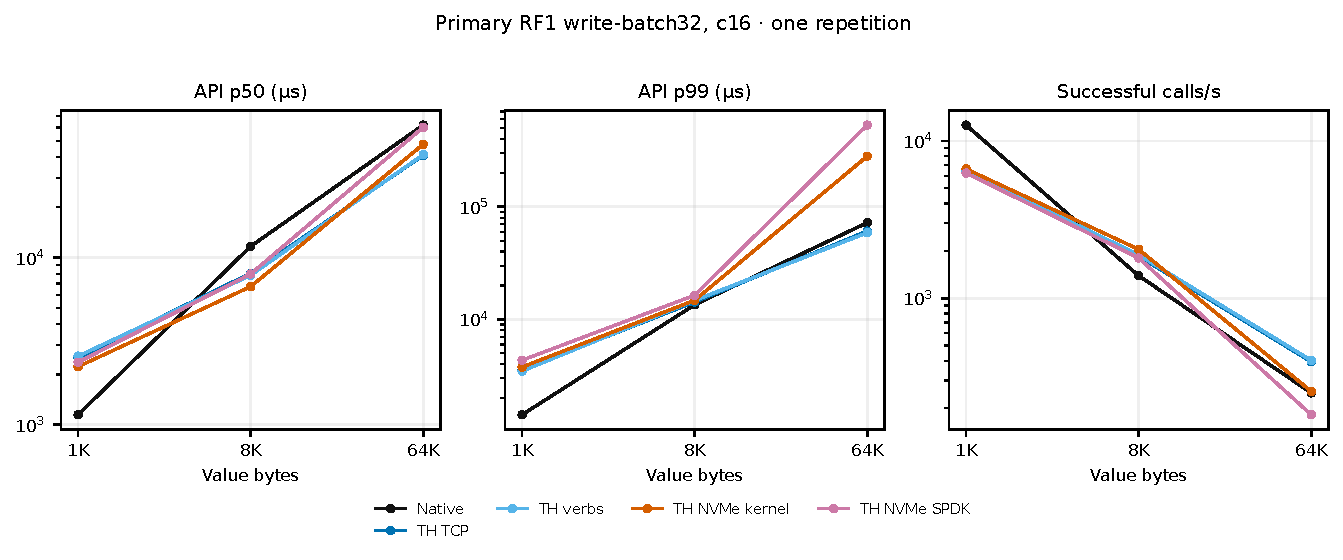
\includegraphics[width=.98\linewidth]{figures/write32.pdf}\\
\small Figure 4. Primary RF1 write-batch32, c16, 2,048 successful calls per case. API p50/p99 and successful calls/s; one repetition. Valkey has no matching batch case; Tidehunter batch durability is not equivalent to scalar write acknowledgements.
\end{center}

\section{Sealed, cold and cached reads}
\begin{center}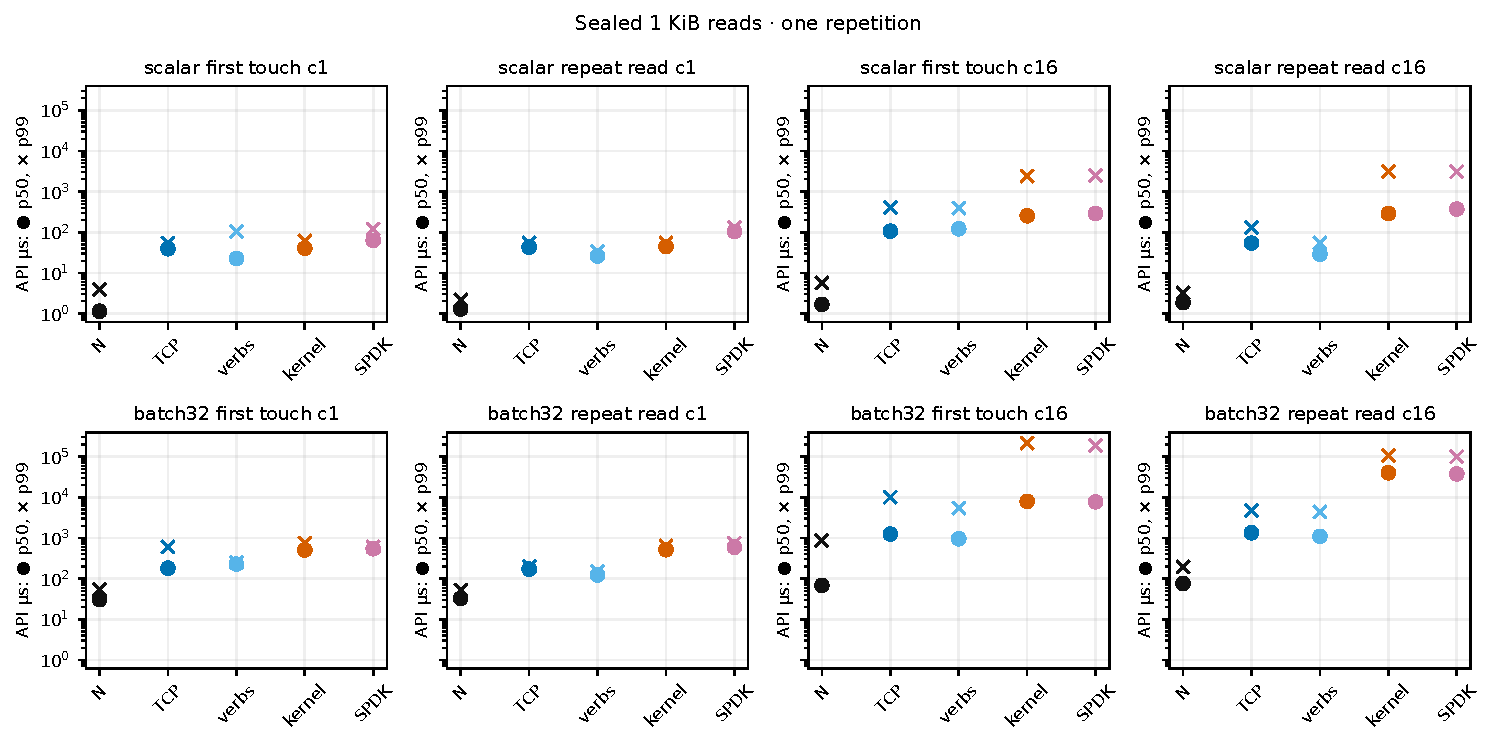
\includegraphics[width=.98\linewidth]{figures/sealed.pdf}\\
\small Figure 5. Sealed 1 KiB first-touch and repeat-read, scalar and batch32, c1 and c16. API p50/p99 of 8,192 scalar or 2,048 batch successful calls per case; one repetition. The first-touch cache drop or eviction is before the measurement gate, not proof of per-call cold access. Kernel buffering and device caches remain. N is native, without network.
\end{center}
\begin{center}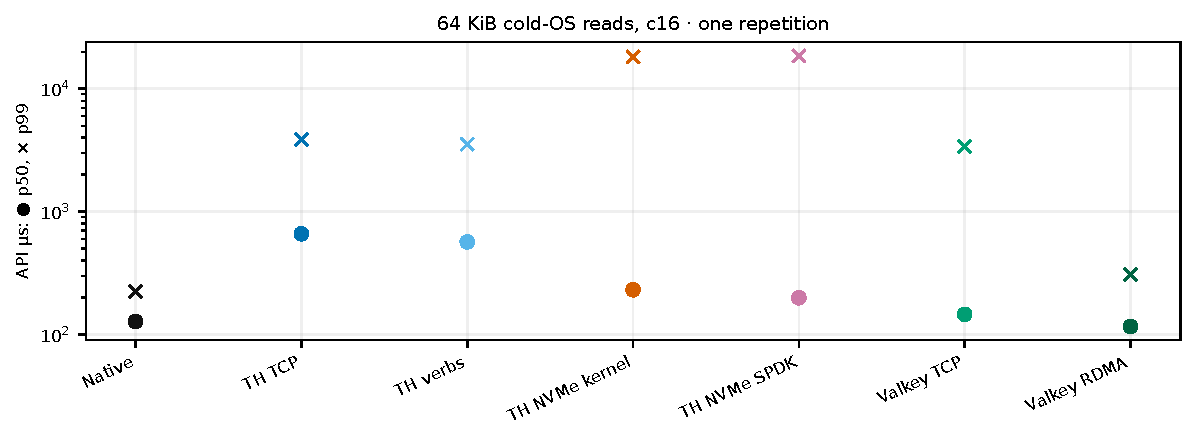
\includegraphics[width=.95\linewidth]{figures/cold.pdf}\\
\small Figure 6. Cold-OS 64 KiB reads, 4,096 successful calls per case; API p50/p99, one repetition. Cache eviction does not prove physical SSD reads; Valkey is RAM-resident. The large tails in cases 0347, 0348 and 0241 remain unexplained and are retained.
\end{center}
\begin{center}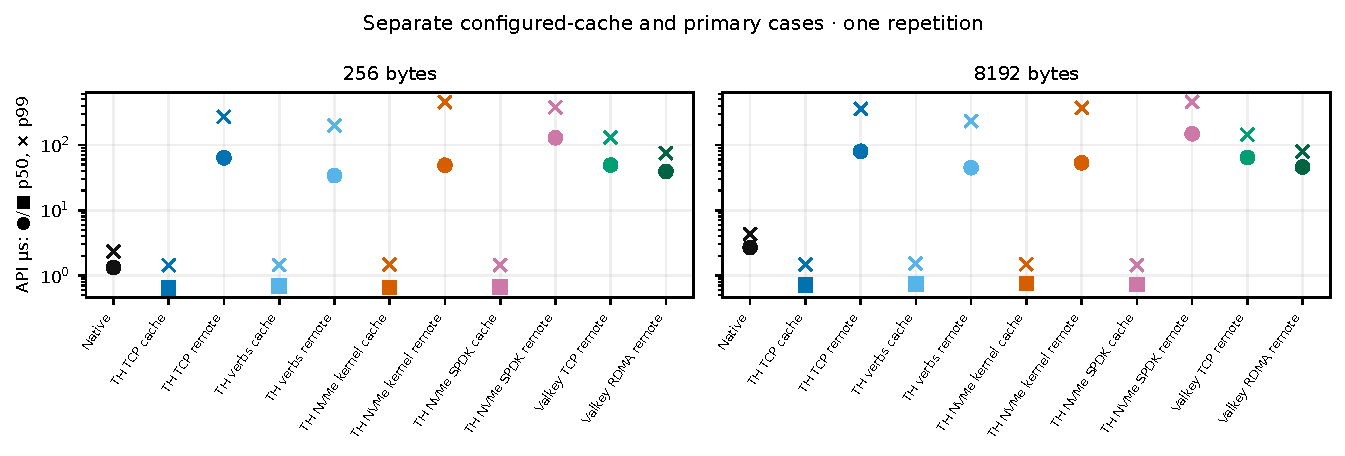
\includegraphics[width=.98\linewidth]{figures/cache.pdf}\\
\small Figure 7. Separate configured-coordinator-cache and primary remote-read cases at 256 B and 8 KiB, 8,192 successful calls per case, API p50/p99, one repetition. Cache-configured does not by itself prove every measured call was a cache hit. Native is local; Valkey uses RAM. These cohorts are not a paired speedup experiment.
\end{center}

\section{Offered load and cross-run context}
\begin{center}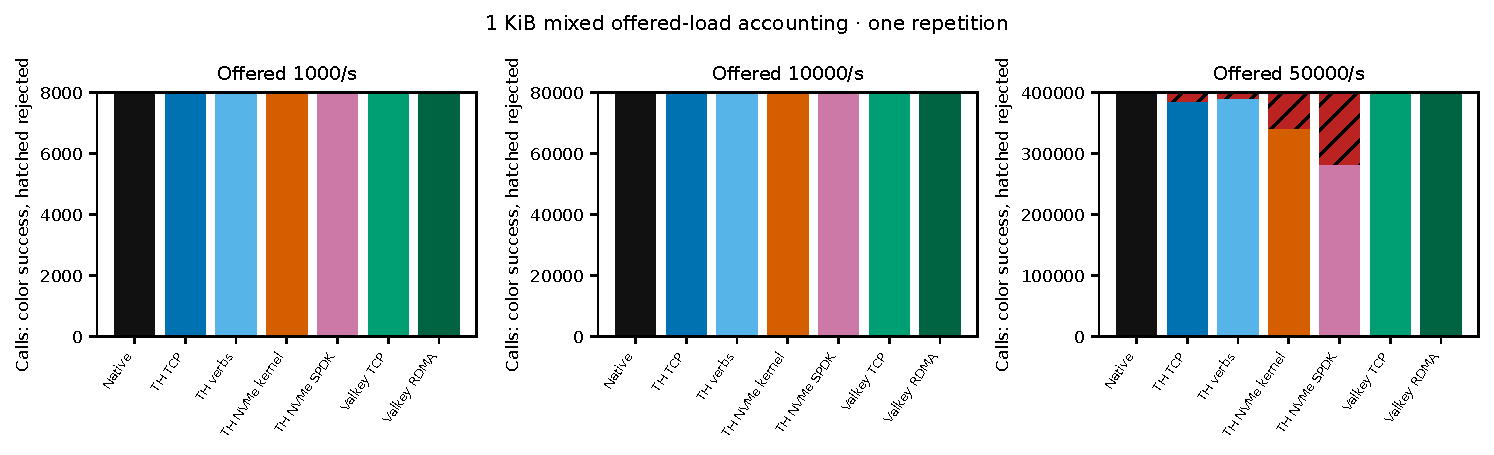
\includegraphics[width=.98\linewidth]{figures/offered.pdf}\\
\small Figure 8. Primary mixed 1 KiB offered-load cases: success and rejected arrivals per whole case, one repetition. The 1,000, 10,000 and 50,000/s cases offer 8,000, 80,000 and 400,000 calls respectively. Counts are not latency; successful API distributions exclude rejections. The 50,000/s cases reject 2,313 Valkey RDMA, 10,291 TH verbs, 14,811 TH TCP, 58,581 kernel and 118,667 SPDK arrivals. Cache and durability contracts differ.
\end{center}
\begin{center}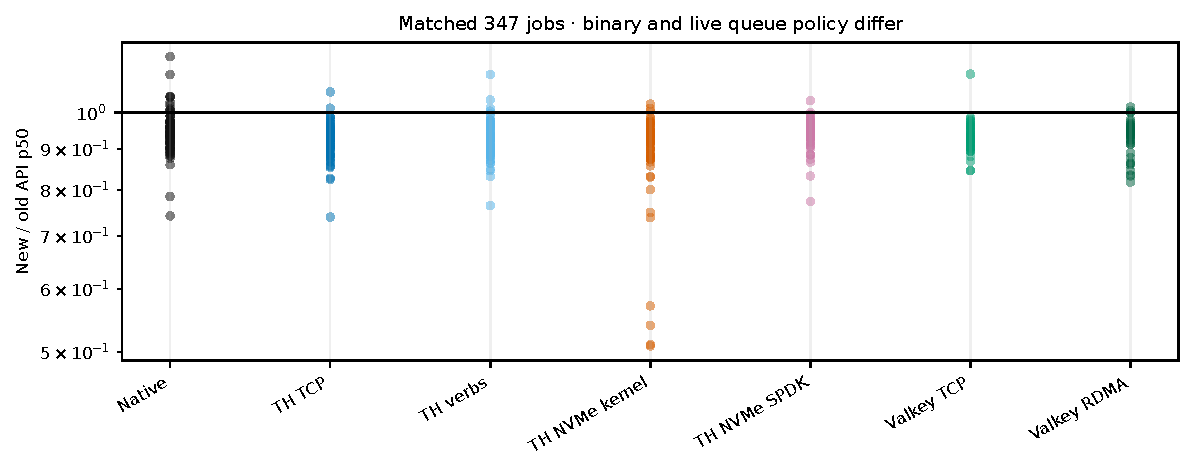
\includegraphics[width=.95\linewidth]{figures/longitudinal.pdf}\\
\small Figure 9. New/old API p50 ratios for each matched successful operation population, without pooling; each point has one repetition in each run and its own sample count in \path{evidence.json}. The 347 matched jobs can yield multiple operation populations. Same hardware class, but binary and run changed; earlier host defaults were 16 by 128 and the new live path requests 1 by 32. The sealed path has no explicit queue flags. Cache and durability settings differ across populations. Ratios cannot attribute cause.
\end{center}
\begin{center}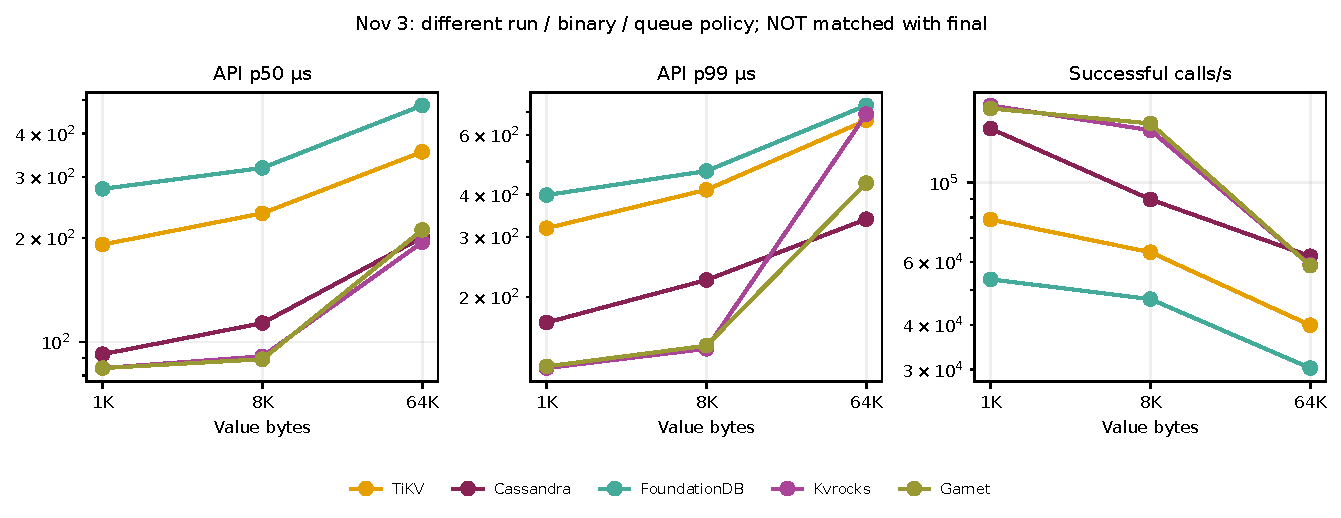
\includegraphics[width=.98\linewidth]{figures/historical-reference.pdf}\\
\small Figure 10. Nov 3 primary RF1 concurrent reads, 8,192 successful calls per case: API p50/p99 and whole-case calls/s, one repetition. Different run, binary and queue policy: not matched with the final run. Cache placement and durability contracts differ across systems. These other KV stores are not final-campaign arms.
\end{center}

\section{Coherence: suspicious orderings}
The recorded populations are numerically coherent, but several orderings are suspicious and unexplained. The rows below are observations, not proven causes or independent experiments; each case has one repetition. Rates are whole-case calls/s. Matched success-population counts are not counts of independent runs.
\begin{center}\small
\begin{tabular}{p{.25\linewidth}p{.66\linewidth}}\toprule
Comparison & Verdict and observed evidence\\\midrule
TH verbs vs TCP & Suspicious: verbs p50 is higher in 19 of 92 matched success populations. At 8 KiB sealed first-touch scalar c1, verbs is 92.804 vs TCP 50.272 \us\ (0086/0056, $n=8192$ each). TCP uses mutual TLS; verbs does not.\\
Valkey RDMA vs TCP & Suspicious: RDMA p50 is higher in 8 of 49 matched success populations. This is not an isolated fabric comparison.\\
Cross-store read & Suspicious as a transport claim: at 64 KiB cold-OS, TH verbs is 565.812 vs Valkey TCP 145.575 \us\ (0183/0241, $n=4096$ each); Valkey GET reads RAM, not the owner WAL.\\
Kernel vs SPDK & Suspicious: at 1 KiB primary live c16, kernel p50 is 46.003 vs SPDK 124.412 \us\ (0327/0328, $n=8192$); buffered and direct target contracts differ.\\
Sealed batch & Suspicious: 1 KiB repeat batch32 kernel c1 is 1,743 calls/s vs c16 369 (0032/0036); c16 repeat p50 is 40.031 ms vs first-touch 7.957 ms (0036/0034), $n=2048$ each. Cache policy and sweep differ.\\
Live writes & Suspicious: 1 KiB c16 live kernel/SPDK p50 is 1.477/1.526 ms vs TH TCP 0.373 ms and Valkey TCP 0.177 ms (0339/0340/0212/0228, $n=4096$ each). Durability contracts differ.\\
Native batch write & Suspicious: 8 KiB native p50 is 11.675 ms vs live kernel 6.707 ms (0263/0325, $n=2048$). Resources and batch implementations differ.\\\bottomrule
\end{tabular}
\end{center}
The coherence grid uses workload, operation and outcome to match cells. All present grid p50 values were checked against the audited population CSV. The differences above do not establish network, queue, storage or persistence as their cause. The native and distributed paths use different resources.

\section{Remote NVMe reads and cache evidence}
The sealed first-touch gate drops or evicts caches before measurement, but that does not prove that measured calls are cold. Owner TCP and verbs may be served by the owner page cache, and native 1 KiB first-touch c1 is only 1.143 \us. The separate cold-OS 64 KiB cohort requests cache drop at read time; it still does not measure the fraction of calls that reach media.

Sealed SPDK has the strongest direct-I/O evidence: a direct-file target, qualified initiator completions and owner bdev completions. This bypasses the target OS page cache, not device or controller caches. At 1 KiB in case 0019, 8,192 initiator completions and 8,192 target bdev completions were recorded; a broader device snapshot reports 8,547 block reads, not a per-call mapping. No per-call NAND-hit fraction or QD=1 disk floor is measured.

\begin{center}\small
\begin{tabular}{lrrrrr}\toprule
Sealed c1 first-touch & Native & TH TCP & TH verbs & Kernel & SPDK\\\midrule
1 KiB & 1.143/3.993 & 39.295/53.919 & 22.716/106.401 & 40.408/61.759 & 62.980/118.948\\
8 KiB & 2.099/5.382 & 50.272/97.142 & 92.804/123.085 & 44.418/83.467 & 106.722/169.056\\
64 KiB & 12.244/372.208 & 97.200/731.471 & 139.192/255.120 & 63.791/376.376 & 137.245/214.749\\\bottomrule
\end{tabular}\\[2pt]
API p50/p99 in \us; $n=8192$ successful calls per case, one repetition. Separate paths and target cache contracts.
\end{center}
In 64 KiB cold-OS c16 ($n=4096$ each), p50 is 127.119 \us\ for native, 658.932 for TCP, 565.812 for verbs, 230.893 for live kernel and 198.806 for live SPDK. Kernel and SPDK p99 are 18.190/18.572 ms and p99.9 are 302.035/432.253 ms. These tails are observed, unexplained and not isolated media latency. Live SPDK target counters cover 1,973 bdev operations versus 4,096 initiator completions in their different observation windows; equality or complete per-call coverage is not established.

\section{Next work: fast remote WAL reads}
\textbf{Decision.} Keep kernel NVMe/RDMA as the current disk-read baseline. Do not claim the present SPDK target is faster: sealed first-touch scalar c1 API p50 at 1/8/64 KiB is 40.408/44.418/63.791 \us\ for kernel and 62.980/106.722/137.245 \us\ for SPDK ($n=8192$ per case). The SPDK arm still uses the kernel initiator and a file-AIO target; the target cache contracts differ. Owner verbs RPC remains a serious alternative for small resident values: its 1 KiB first-touch p50 is 22.716 \us\ in case 0038, not a proven device-read floor.

\textbf{First experiment, E0.} Measure a controlled QD=1 floor before selecting an optimization: compare fio over NVMe/RDMA, local SPDK bdevperf and our checksum-owning client against explicitly identified backends. Match transfer size, device ownership, cache state and CPU placement where possible. Record effective queue geometry, requested and completed depth, host and target block activity, and latency distributions. The local bdevperf result is a component baseline, not the same end-to-end operation; separate path and cache contracts. Repeat independently and preserve tails and errors.

\textbf{Ranked options.} Each item below is an \textbf{[INFERENCE]} design estimate, not a measured improvement or a numerical promise. Isolate each change against E0 and loaded controls; retain exact-reference checks, CRC, fencing, authority and DMA-buffer lifetimes.
\begin{enumerate}\setlength{\itemsep}{1pt}\setlength{\parskip}{0pt}
\item One bounded progress owner per controller or CPU; allow multiple flights and remove avoidable lane blocking and shared-reader contention.
\item Prototype an SPDK NVMe/RDMA initiator with owned polling qpairs, then compare it with the optimized kernel initiator.
\item Compare the current file-AIO backing bdev with file-uring and, only on exclusively owned disposable storage, native SPDK NVMe.
\item Register fixed aligned buffers and files; remove the live member \texttt{.to\_vec()} copy with a lifetime-safe retained buffer. Sealed extraction already avoids that copy.
\item Merge duplicate or overlapping authorized aligned ranges, then verify and slice every member.
\item Isolate progress and target CPUs and place memory and interrupt work deliberately by NUMA node.
\item Sweep bounded queue counts and depths, measuring effective controller geometry, memory registration pressure, goodput and p99.
\item Test SQPOLL with fixed buffers and controlled CPU cost; it changes submission, not target or device polling.
\item Feature-probe RDMA polling queues and IOPOLL, and separately probe namespace \texttt{uring\_cmd}; do not assume deployed-kernel support.
\item Pre-open the next known WAL file grant when miss and setup measurements justify it; keep pins and controller use bounded.
\item Test bounded reference prefetch with demand priority and count useful, late and wasted reads.
\item Evaluate the existing coordinator RAM cache and, separately, a registered-RAM tier; a hit avoids storage work and is not a faster disk read.
\end{enumerate}
\textbf{Do not pursue as shortcuts.} Do not cargo-cult \texttt{inline\_data\_size} for READ replies, blindly restore 16-by-128 queues, call a CQ peek device polling, or treat an mmap registration as SSD-as-RDMA. PMEM, controller memory buffers and peer-to-peer DMA need unproved hardware and ownership support; do not use a fixed batching delay on the latency-critical path. Preserve the write durability contract.

\textbf{Unknowns and acceptance.} The true QD=1 floors, sealed controller queue geometry, causes of the 0347/0348 tails, actual IRDMA capabilities, CIQ 5.14 IOPOLL support and a representative Sui trace remain open. Accept a change only after repeated, same-contract comparisons with explicit cache and security settings, bounded resource cost, correct data and no hidden rejection or p99 regression. The design evidence and proposed experiment details are under \path{analysis/nvme-design/} in the campaign directory.

\section{Provenance and limits}
The admitted terminal archive SHA-256 is \path{6070cbc80a63109006cc33381dbd9d798ac0442940941f45b9851560fe7dc1a0}. The figure script reads the audited all-populations CSV and the matched longitudinal CSV, plus the Nov 3 reference CSV. \path{evidence.json} records source hashes, figure hashes, case identifiers, population counts and source values. The raw archive, complete measurement tables and campaign report are under \path{checkpoint-work/spdk-matched-storage-20261105T004442Z/}. Four native Valkey controls are separate histogram-based benchmarks, not pooled with API populations. No claim about Sui, physical NAND time, isolated network time or statistical significance follows from these measurements.
The coherence grid and anomaly inventory are in \path{analysis/coherence/} and the remote storage evidence is in \path{analysis/remote-nvme/} under that campaign directory. Live queue options are set in \path{tidehunter/src/distributed/nvmeof/live_connect.rs}; the sealed connection is made via \path{experiments/nvmeof/campaign_targets.py} and \path{manage.py} without queue flags.

\begin{thebibliography}{9}\small
\bibitem{tidehunter} A. Chursin et al., \emph{Tidehunter: Large-Value Storage With Minimal Data Relocation}, \href{https://arxiv.org/abs/2602.01873v2}{arXiv:2602.01873v2}.
\end{thebibliography}
\clearpage
\appendix
\section{Full 1, 8 and 64 KiB comparison}
Each entry is API p50/p99 in \us\ followed by successful calls/s. Primary live, native and Valkey cells are c16, RF1; scalar read $n=8192$, scalar write $n=4096$, and batch $n=2048$. Sealed cells are separate first-touch c16 read cases, not matched to primary live; they have the same per-operation counts. Sealed writes were not measured in this cohort, and 64 KiB sealed c16 cases are absent. Valkey write-batch32 is unsupported. A dash means no comparable case, not zero. One repetition; cache, resource and persistence contracts differ.
\begin{center}\scriptsize
\resizebox{\linewidth}{!}{%
\begin{tabular}{lrrrr}\toprule
Backend & Scalar read & Scalar write & Read-many32 & Write-batch32\\\midrule
Native & 1.5/2.6/270631 & 68.7/169.6/157365 & 64.5/103.8/98852 & 1148.5/1425.0/12605\\
TH TCP & 63.6/283.5/160111 & 373.2/906.3/38490 & 1252.1/3781.5/10868 & 2522.9/3561.8/6495\\
TH verbs & 35.8/191.2/239334 & 361.9/833.5/39462 & 1126.0/3707.8/11563 & 2573.5/3474.2/6426\\
NVMe kernel live & 46.0/373.3/111589 & 1477.4/4323.2/9198 & 1187.8/4570.2/10566 & 2226.3/3777.2/6636\\
NVMe kernel sealed & 254.1/2412.7/35862 & -- & 7956.8/214410.2/586 & --\\
NVMe SPDK live & 124.4/380.7/97561 & 1525.9/4132.6/8959 & 1332.3/6356.7/8975 & 2364.5/4339.4/6248\\
NVMe SPDK sealed & 287.4/2503.3/33364 & -- & 7721.3/191637.3/626 & --\\
Valkey TCP & 49.5/94.9/200965 & 177.2/438.0/78150 & 372.7/797.1/31498 & --\\
Valkey RDMA & 41.2/92.5/150160 & 172.9/439.6/80146 & 320.7/788.2/35821 & --\\
\bottomrule\end{tabular}}\\[3pt]
1 KiB: successful API p50/p99 (\us) / calls per second.
\end{center}
\begin{center}\scriptsize
\resizebox{\linewidth}{!}{%
\begin{tabular}{lrrrr}\toprule
Backend & Scalar read & Scalar write & Read-many32 & Write-batch32\\\midrule
Native & 2.7/4.3/305956 & 230.5/387.4/62567 & 81.9/258.8/45566 & 11675.4/13482.1/1390\\
TH TCP & 80.0/356.5/117956 & 553.4/1441.8/26211 & 1392.0/4946.9/9150 & 8060.2/14283.8/1848\\
TH verbs & 44.8/231.3/197619 & 582.4/1024.6/25865 & 1171.3/3320.8/10622 & 7843.1/14726.1/1888\\
NVMe kernel live & 53.3/369.6/102897 & 1679.1/4562.7/8418 & 1243.2/9625.6/8797 & 6707.2/14770.0/2045\\
NVMe kernel sealed & 295.9/2368.8/32874 & -- & 8226.7/196691.3/630 & --\\
NVMe SPDK live & 148.2/459.5/67086 & 1774.9/4758.0/7894 & 1384.5/21671.7/7394 & 7980.6/16382.0/1803\\
NVMe SPDK sealed & 313.3/2327.7/32399 & -- & 7925.0/174969.6/666 & --\\
Valkey TCP & 64.1/142.7/155699 & 224.8/534.7/61155 & 517.9/198143.5/3332 & --\\
Valkey RDMA & 45.9/80.2/142170 & 216.9/520.8/63414 & 375.5/1148.9/21097 & --\\
\bottomrule\end{tabular}}\\[3pt]
8 KiB: successful API p50/p99 (\us) / calls per second.
\end{center}
\begin{center}\scriptsize
\resizebox{\linewidth}{!}{%
\begin{tabular}{lrrrr}\toprule
Backend & Scalar read & Scalar write & Read-many32 & Write-batch32\\\midrule
Native & 14.8/26.3/199283 & 2934.9/3543.0/5738 & 1252.9/7879.7/2544 & 62053.2/72191.7/250\\
TH TCP & 163.3/723.7/50613 & 1629.9/3158.9/9168 & 5857.4/15312.9/1725 & 40909.5/60727.2/394\\
TH verbs & 82.2/339.8/99756 & 1632.0/3175.0/9073 & 1658.2/33731.3/3594 & 41336.3/58792.8/403\\
NVMe kernel live & 94.9/270.8/65193 & 2144.4/6711.8/6302 & 1784.4/37827.1/3115 & 47645.1/280717.5/256\\
NVMe kernel sealed & -- & -- & -- & --\\
NVMe SPDK live & 193.2/590.4/48302 & 2629.8/8089.9/5254 & 2100.9/39674.1/2829 & 60180.7/530516.3/182\\
NVMe SPDK sealed & -- & -- & -- & --\\
Valkey TCP & 144.1/3173.4/21940 & 444.3/1254.9/29605 & 4431.8/365683.8/243 & --\\
Valkey RDMA & 117.2/276.0/82860 & 418.7/1119.7/31902 & 1439.9/43334.1/2159 & --\\
\bottomrule\end{tabular}}\\[3pt]
64 KiB: successful API p50/p99 (\us) / calls per second.
\end{center}

\end{document}
